
\question
If $a(t)=4 t-1$ and $v(1)=3$, then $v(t)$ equals
\begin{choices}
  \choice $2 t^{2}-t$
  \choice $2 t^{2}-t+1$
  \CorrectChoice $2 t^{2}-t+2$
  \choice $2 t^{2}+1$
  \choice $2 t^{2}+2$
\end{choices}
\begin{solution}
$v(t)=2 t^{2}-t+C ; v(1)=3$; so $C=2$.
\end{solution}

\question\label{calc09:motion-v-s}
If $a(t)=20 t^{3}-6 t, s(-1)=2$, and $s(1)=4$, then $v(t)$ equals
\begin{choices}
  \choice $t^{5}-t^{3}$
  \CorrectChoice $5 t^{4}-3 t^{2}+1$
  \choice $5 t^{4}-3 t^{2}+3$
  \choice $t^{5}-t^{3}+t+3$
  \choice $t^{5}-t^{3}+1$
\end{choices}
\begin{solution}
If $a(t)=20 t^{3}-6 t$, then
\[
\begin{gathered}
v(t)=5 t^{4}-3 t^{2}+C_{1} \\
s(t)=t^{5}-t^{3}+C_{1} t+C_{2}
\end{gathered}
\]
Since
\[
s(-1)=-1+1-C_{1}+C_{2}=2
\]
and
\[
s(1)=1-1+C_{1}+C_{2}=4,
\]
therefore
\[
\begin{gathered}
2 C_{2}=6, C_{2}=3 \\
C_{1}=1
\end{gathered}
\]
So
\[
v(t)=5 t^{4}-3 t^{2}+1
\]
\end{solution}


\newpage




\question
Given $a(t), s(-1)$, and $s(1)$ as in Question~\ref{calc09:motion-v-s}, then $s(0)$ equals
\begin{choices}
  \choice 0
  \choice 1
  \choice 2
  \CorrectChoice 3
  \choice 4
\end{choices}
\begin{solution}
From Question~\ref{calc09:motion-v-s}, $s(t)=t^{5}-t^{3}+t+3$, so $s(0)=C_{2}=3$.
\end{solution}

\question\label{calc09:stone-building}
A stone is thrown straight up from the top of a building with initial velocity $40 \mathrm{ft} / \mathrm{sec}$ and hits the ground 4 sec later. The height of the building, in feet, is
\begin{choices}
  \choice 88
  \CorrectChoice 96
  \choice 112
  \choice 128
  \choice 144
\end{choices}
\begin{solution}
Since $a(t)=-32, v(t)=-32 t+40$, and the height of the stone $s(t)=-16 t^{2}+40 t+C$. When the stone hits the ground, 4 sec later, $s(t)=0$, so


\[
\begin{aligned}
& 0=-16(16)+40(4)+C \\
& C=96 \mathrm{ft}
\end{aligned}
\]


\end{solution}

\question
The maximum height is reached by the stone in Question~\ref{calc09:stone-building} after
\begin{choices}
  \choice $4 / 5 \mathrm{sec}$
  \choice 4 sec
  \CorrectChoice $5 / 4 \mathrm{sec}$
  \choice $5 / 2 \mathrm{sec}$
  \choice 2 sec
\end{choices}
\begin{solution}
From Question~\ref{calc09:stone-building}
\[
s(t)=-16 t^{2}+40 t+96
\]
Then
\[
s^{\prime}(t)=-32 t+40
\]
which is zero if $t=5 / 4$, and that yields maximum height, since $s^{\prime \prime}(t)=-32$.
\end{solution}


\newpage



\question
If a car accelerates from 0 to 60 mph in 10 sec , what distance does it travel in those 10 sec ? (Assume the acceleration is constant and note that $60 \mathrm{mph}=88 \mathrm{ft} / \mathrm{sec}$.)
\begin{choices}
  \choice 40 ft
  \choice 44 ft
  \choice 88 ft
  \choice 400 ft
  \CorrectChoice 440 ft
\end{choices}
\begin{solution}
(E) The velocity $v(t)$ of the car is linear, since its acceleration is constant and

\[
a=\dfrac{d v}{d t}=\dfrac{88 \mathrm{ft} / \mathrm{sec}}{10 \mathrm{sec}}=8.8 \mathrm{ft} / \mathrm{sec}^{2}
\]

so $v(t)=8.8 t$ and $s(t)=4.4 t^{2}$; hence $s(10)=440$ ft.
\end{solution}

\question
A stone is thrown at a target so that its velocity after $t \mathrm{sec}$ is $(100-20 t) \mathrm{ft} / \mathrm{sec}$. If the stone hits the target in 1 sec , then the distance from the sling to the target is
\begin{choices}
  \choice 80 ft
  \CorrectChoice 90 ft
  \choice 100 ft
  \choice 110 ft
  \choice 120 ft
\end{choices}
\begin{solution}
(B) Since $v=100-20 t, s=100 t-10 t^{2}+C$ with $s(0)=0$. So $s(1)=100-10=$ 90 ft .
\end{solution}

\question
What should the initial velocity be if you want a stone to reach a height of 100 ft when you throw it straight up?
\begin{choices}
  \CorrectChoice $80 \mathrm{ft} / \mathrm{sec}$
  \choice $92 \mathrm{ft} / \mathrm{sec}$
  \choice $96 \mathrm{ft} / \mathrm{sec}$
  \choice $112 \mathrm{ft} / \mathrm{sec}$
  \choice none of these
\end{choices}
\begin{solution}
(A) Since $v=-32 t+v_{0}$ and $s=-16 t^{2}+v_{0} t$, we solve simultaneously:
\[
\begin{aligned}
0 & =-32 t+v_{0} \\
100 & =-16 t^{2}+v_{0} t
\end{aligned}
\]
These yield $t=5 / 2$ and $v_{0}=80 \mathrm{ft} / \mathrm{sec}$.
\end{solution}


\newpage


\question\label{calc09:odometer}
If the velocity of a car traveling in a straight line at time $t$ is $v(t)$, then the difference in its odometer readings between times $t=a$ and $t=b$ is
\begin{choices}
  \CorrectChoice $\int_{a}^{b}|v(t)| d t$
  \choice $\int_{a}^{b} v(t) d t$
  \choice the net displacement of the car's position from $t=a$ to $t=b$
  \choice the change in the car's position from $t=a$ to $t=b$
  \choice none of these
\end{choices}
\begin{solution}
(A) The odometer measures the total trip distance from time $t=a$ to $t=b$ (whether the car moves forward or backward or reverses its direction one or more times from $t=a$ to $t=b$ ). This total distance is given exactly by $\int_{a}^{b}|v(t)| d t$.
\end{solution}

\question
If an object is moving up and down along the $y$-axis with velocity $v(t)$ and $s^{\prime}(t)=v(t)$, then it is false that $\int_{a}^{b} v(t) d t$ gives
\begin{choices}
  \choice $s(b)-s(a)$
  \choice the net distance traveled by the object between $t=a$ and $t=b$
  \choice the total change in $s(t)$ between $t=a$ and $t=b$
  \choice the shift in the object's position from $t=a$ to $t=b$
  \CorrectChoice the total distance covered by the object from $t=a$ to $t=b$
\end{choices}
\begin{solution}
(E) (A), (B), (C), and (D) are all true. (E) is false: see Question~\ref{calc09:odometer}.
\end{solution}

\question\label{calc09:separable-ydyx}
Solutions of the differential equation $y d y=x d x$ are of the form
\begin{choices}
  \CorrectChoice $x^{2}-y^{2}=C$
  \choice $x^{2}+y^{2}=C$
  \choice $y^{2}=C x^{2}$
  \choice $x^{2}-C y^{2}=0$
  \choice $x^{2}=C-y^{2}$
\end{choices}
\begin{solution}
(A) Integrating yields $\dfrac{y^{2}}{2}=\dfrac{x^{2}}{2}+C$ or $y^{2}=x^{2}+2 C$ or $y^{2}=x^{2}+C^{\prime}$, where we have replaced the arbitrary constant $2 C$ by $C^{\prime}$.
\end{solution}


\newpage



\question
Find the domain of the particular solution to the differential equation in Question~\ref{calc09:separable-ydyx} that passes through point $(-2,1)$.
\begin{choices}
  \choice $x<0$
  \choice $-2 \leq x<0$
  \CorrectChoice $x<-\sqrt{3}$
  \choice $|x|<\sqrt{3}$
  \choice $|x|>\sqrt{3}$
\end{choices}
\begin{solution}
(C) For initial point $(-2,1), x^{2}-y^{2}=3$. Rewriting the d.e. $y d y=x d x$ as $\dfrac{d y}{d x}=\dfrac{x}{y}$ reveals that the derivative does not exist when $y=0$, which occurs at $x= \pm \sqrt{3}$. Since the particular solution must be differentiable in an interval containing $x=-2$, the domain is $x<-\sqrt{3}$.
\end{solution}

\question
If $\dfrac{d y}{d x}=\dfrac{y}{2 \sqrt{x}}$ and $y=1$ when $x=4$, then
\begin{choices}
  \choice $y^{2}=4 \sqrt{x}-7$
  \choice $\ln y=4 \sqrt{x}-8$
  \choice $\ln y=\sqrt{x-2}$
  \choice $y=e^{\sqrt{x}}$
  \CorrectChoice $y=e^{\sqrt{x}-2}$
\end{choices}
\begin{solution}
(E) We separate variables. $\int \dfrac{d y}{y}=\dfrac{1}{2} \int x^{-\dfrac{1}{2}} d x$, so $\ln |y|=\sqrt{x}+c$. The initial point yields $\ln 1=\sqrt{4}+c$; hence $c=-2$. With $y>0$, the particular solution is $\ln y=\sqrt{x}-2$, or $y=e^{\sqrt{x}-2}$.
\end{solution}

\question
If $\dfrac{d y}{d x}=e^{y}$ and $y=0$ when $x=1$, then
\begin{choices}
  \choice $y=\ln |x|$
  \choice $y=\ln |2-x|$
  \CorrectChoice $e^{-y}=2-x$
  \choice $y=-\ln |x|$
  \choice $e^{-y}=x-2$
\end{choices}
\begin{solution}
(C) We separate variables. $\int e^{-y} d y=\int d x$, so $-e^{-y}=x+c$. The particular solution is $-e^{-y}=x-2$.
\end{solution}


\newpage



\question
If $\dfrac{d y}{d x}=\dfrac{x}{\sqrt{9+x^{2}}}$ and $y=5$ when $x=4$, then $y$ equals
\begin{choices}
  \choice $\sqrt{9+x^{2}}-5$
  \CorrectChoice $\sqrt{9+x^{2}}$.
  \choice $2 \sqrt{9+x^{2}}-5$
  \choice $\dfrac{\sqrt{9+x^{2}}+5}{2}$
  \choice none of these
\end{choices}
\begin{solution}
(B) The general solution is $y=\dfrac{1}{2} \int\left(9+x^{2}\right)^{-\dfrac{1}{2}}(2 x d x)=\sqrt{9+x^{2}}+C ; y=5$ when $x=4$ yields $C=0$.
\end{solution}

\question
The general solution of the differential equation $x d y=y d x$ is a family of
\begin{choices}
  \choice circles
  \choice hyperbolas
  \choice parallel lines
  \choice parabolas
  \CorrectChoice lines passing through the origin
\end{choices}
\begin{solution}
(E) Since $\int \dfrac{d y}{y}=\int \dfrac{d x}{x}$, it follows that

\[
\ln y=\ln x+C \quad \text { or } \quad \ln y=\ln x+\ln k ;
\]

so $y=k x$.
\end{solution}

\question
The general solution of the differential equation $\dfrac{d y}{d x}=y$ is a family of
\begin{choices}
  \choice parabolas
  \choice straight lines
  \choice hyperbolas
  \choice ellipses
  \CorrectChoice none of these
\end{choices}
\begin{solution}
(E) $\quad \int \dfrac{d y}{y}=\int d x$ yields $\ln |y|=x+c$; hence the general solution is $y=k e^{x}, k \neq 0$.
\end{solution}


\newpage



\question
A function $f(x)$ that satisfies the equations $f(x) f^{\prime}(x)=x$ and $f(0)=1$ is
\begin{choices}
  \CorrectChoice $f(x)=\sqrt{x^{2}+1}$
  \choice $f(x)=\sqrt{1-x^{2}}$.
  \choice $f(x)=x$
  \choice $f(x)=e^{x}$
  \choice none of these
\end{choices}
\begin{solution}
(A) We rewrite and separate variables, getting $y \dfrac{d y}{d x}=x$. The general solution is

\[
y^{2}=x^{2}+C \quad \text { or } \quad f(x)= \pm \sqrt{x^{2}+C}
\]


\end{solution}

\question\label{calc09:curve-3y-x}
The curve that passes through the point $(1,1)$ and whose slope at any point $(x, y)$ is equal to $\dfrac{3 y}{x}$ has the equation
\begin{choices}
  \choice $3 x-2=y$
  \choice $y^{3}=x$
  \CorrectChoice $y=x^{3}$
  \choice $3 y^{2}=x^{2}+2$
  \choice $3 y^{2}-2 x=1$
\end{choices}
\begin{solution}
We are given that $\dfrac{d y}{d x}=\dfrac{3 y}{x}$. The general solution is $\ln |y|=3 \ln |x|+C$.


Thus, $|y|=c\left|x^{3}\right| ; y= \pm c x^{3}$. Since $y=1$ when $x=1$, we get $c=1$.
\end{solution}

\question
What is the domain of the particular solution in Question~\ref{calc09:curve-3y-x}?
\begin{choices}
  \choice all real numbers
  \choice $|x| \leq 1$
  \choice $x \neq 0$
  \choice $x<0$
  \CorrectChoice $x>0$
\end{choices}
\begin{solution}
(E) The d.e. $\dfrac{d y}{d x}=\dfrac{3 y}{x}$ reveals that the derivative does not exist when $x=0$.

Since the particular solution must be differentiable in an interval containing initial value $x=1$, the domain is $x>0$.
\end{solution}


\newpage



\question
If $\dfrac{d y}{d x}=\dfrac{k}{x}, k$ a constant, and if $y=2$ when $x=1$ and $y=4$ when $x=e$, then, when $x=2, y$ equals
\begin{choices}
  \choice 2
  \choice 4
  \choice $\ln 8$
  \choice $\ln 2+2$
  \CorrectChoice $\ln 4+2$
\end{choices}
\begin{solution}
(E) The general solution is $y=k \ln |x|+C$, and the particular solution is $y=2 \ln |x|+2$.
\end{solution}


\newpage



\question
The slope field shown at the right is for the differential equation
\begin{center}
  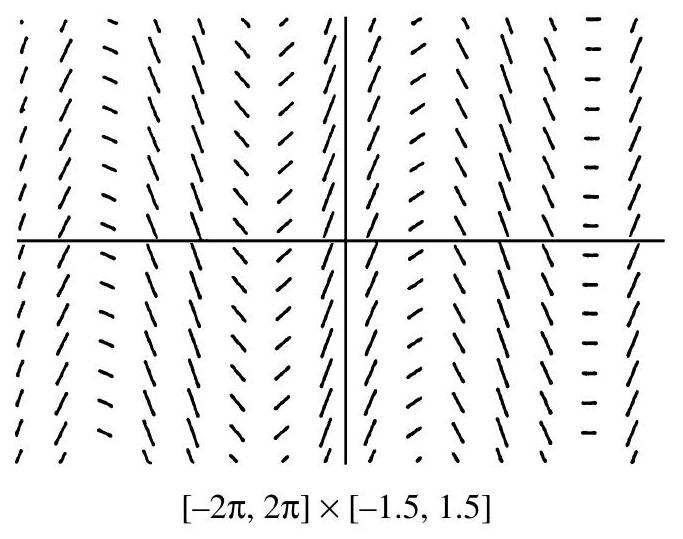
\includegraphics[width=0.50\linewidth]{calculus/images/bfd66936-4ec5-43f7-bf96-19a19e48d25c-03_539_683_1677_995.jpg}
\end{center}
\begin{choices}
  \choice $y^{\prime}=x+1$
  \choice $y^{\prime}=\sin x$
  \choice $y^{\prime}=-\sin x$
  \CorrectChoice $y^{\prime}=\cos x$
  \choice $y^{\prime}=-\cos x$
\end{choices}
\begin{solution}
(D) We carefully(!) draw a curve for a solution to the d.e. represented by the slope field. It will be the graph of a member of the family $y=\sin x+C$. At the right we have superimposed the graph of the particular solution $y=\sin x-0.5$.
\begin{center}
  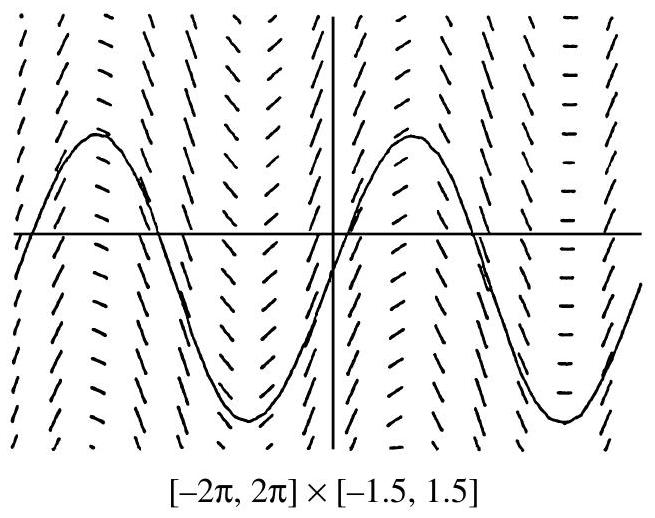
\includegraphics[width=0.50\linewidth]{calculus/images/bfd66936-4ec5-43f7-bf96-19a19e48d25c-11_518_655_881_1025.jpg}
\end{center}
\end{solution}


\newpage



\question
The slope field at the right is for the differential equation
\begin{center}
  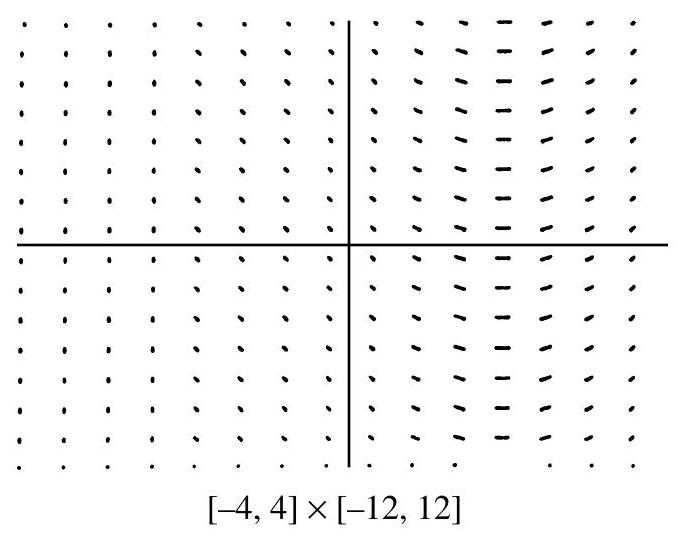
\includegraphics[width=0.50\linewidth]{calculus/images/bfd66936-4ec5-43f7-bf96-19a19e48d25c-03_541_685_2231_997.jpg}
\end{center}
\begin{choices}
  \choice $y^{\prime}=2 x$
  \CorrectChoice $y^{\prime}=2 x-4$
  \choice $y^{\prime}=4-2 x$
  \choice $y^{\prime}=y$
  \choice $y^{\prime}=x+y$
\end{choices}
\begin{solution}
(B)
\begin{center}
  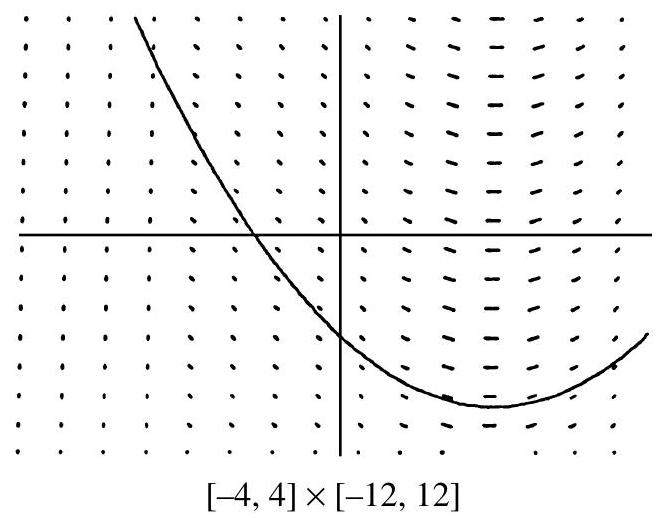
\includegraphics[width=0.50\linewidth]{calculus/images/bfd66936-4ec5-43f7-bf96-19a19e48d25c-11_518_665_1447_658.jpg}
\end{center}
It's easy to see that the answer must be choice (A), (B), or (C), because the slope field depends only on $x$ : all the slope segments for a given $x$ are parallel. Also, the solution curves in the slope field are all concave up, as they are only for choices (A) and (B). Finally, the solution curves all have a minimum at $x=2$, which is true only for differential equation (B).
\end{solution}



\newpage



\question
A solution curve has been superimposed on the slope field shown at the right. The solution is for the differential equation and initial condition
\begin{center}
  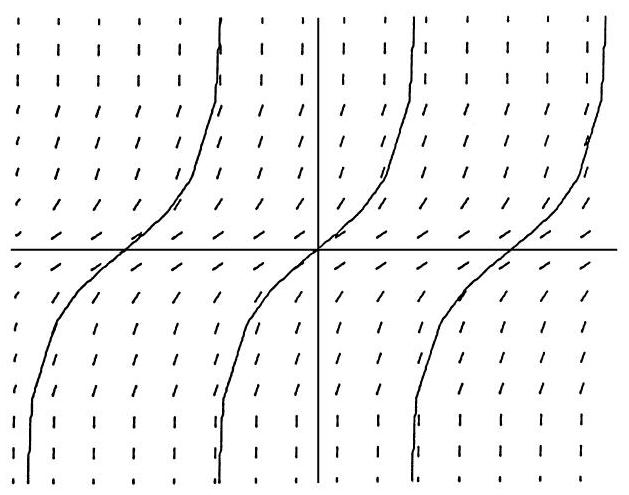
\includegraphics[width=0.50\linewidth]{calculus/images/bfd66936-4ec5-43f7-bf96-19a19e48d25c-04_495_629_343_1410.jpg}
\end{center}
\begin{choices}
  \choice $y^{\prime}=\tan x ; y(0)=0$
  \choice $y^{\prime}=\cot x, y(\pi / 4)=1$
  \choice $y^{\prime}=1+x^{2} ; y(0)=0$
  \choice $y^{\prime}=\dfrac{1}{1+x^{2}} ; y\left(\dfrac{\pi}{4}\right)=1$
  \CorrectChoice $y^{\prime}=1+y^{2} ; y(0)=0$
\end{choices}
\begin{solution}
(E) The solution curve is $y=\tan x$, which we can obtain from the differential equation $y^{\prime}=1+y^{2}$ with the condition $y(0)=0$ as follows:
\[
\dfrac{d y}{1+y^{2}}=d x, \quad \tan ^{-1} y=x, \quad y=\tan x+C
\]
Since $y(0)=0, C=0$. Verify that (A) through (D) are incorrect.
\end{solution}




\newpage



\begin{EnvFullwidth}
\textit{The slope fields below are for Questions~\ref{calc09:slope-first}--\ref{calc09:slope-last}.}

NOTE: In matching slope fields and differential equations in Questions~\ref{calc09:slope-first}--\ref{calc09:slope-last}, keep in mind that if the slope segments along a vertical line are all parallel, signifying equal slopes for a fixed $x$, then the differential equation can be written as $y^{\prime}=f(x)$. Replace ``vertical'' by ``horizontal'' and ``$x$'' by ``$y$'' in the preceding sentence to obtain a differential equation of the form $y^{\prime}=g(y)$.
\begin{center}
  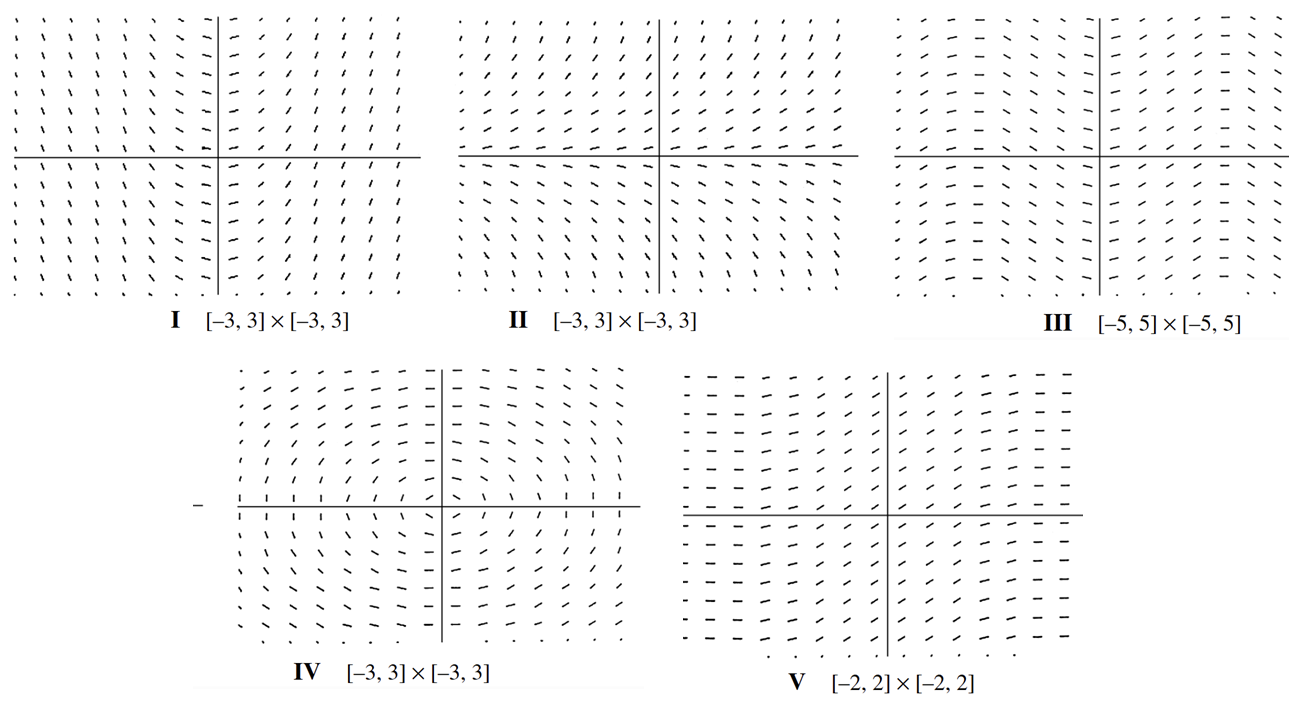
\includegraphics[width=\linewidth]{calculus/images/more02.png}
\end{center}
\end{EnvFullwidth}

\question\label{calc09:slope-first}
Which slope field is for the differential equation $y^{\prime}=y$ ?
\begin{choices}
  \choice I
  \CorrectChoice II
  \choice III
  \choice IV
  \choice V
\end{choices}
\begin{solution}
(B) The slope field for $y^{\prime}=y$ must by II; it is the only one whose slopes are equal along a horizontal line.
\end{solution}



\newpage



\question
Which slope field is for the differential equation $y^{\prime}=-\dfrac{x}{y}$ ?
\begin{choices}
  \choice I
  \choice II
  \choice III
  \CorrectChoice IV
  \choice V
\end{choices}
\begin{solution}
(D) Of the four remaining slope fields, IV is the only one whose slopes are not equal along either a vertical or a horizontal line (the segments are not parallel). Its d.e. therefore cannot be either of type $y^{\prime}=f(x)$ or $y^{\prime}=g(y)$. The d.e. must be implicitly defined-that is, of the form $y^{\prime}=F(x, y)$. So the answer here is IV.
\end{solution}

\question
Which slope field is for the differential equation $y^{\prime}=\sin x$ ?
\begin{choices}
  \choice I
  \choice II
  \CorrectChoice III
  \choice IV
  \choice V
\end{choices}
\begin{solution}
(C) The remaining slope fields, I, III, and V, all have d.e.'s of the type $y^{\prime}=f(x)$. The curves "lurking" in III are trigonometric curves-not so in I and V.
\end{solution}

\question
Which slope field is for the differential equation $y^{\prime}=2 x$ ?
\begin{choices}
  \CorrectChoice I
  \choice II
  \choice III
  \choice IV
  \choice V
\end{choices}
\begin{solution}
(A) Given $y^{\prime}=2 x$, we immediately obtain the general solution, a family of parabolas, $y=x^{2}+C$. (Trace the parabola in I through ( 0,0 ), for example.)
\end{solution}




\newpage



\question\label{calc09:slope-last}
Which slope field is for the differential equation $y^{\prime}=e^{-x^{2}}$ ?
\begin{choices}
  \choice I
  \choice II
  \choice III
  \choice IV
  \CorrectChoice V
\end{choices}
\begin{solution}
(E) V is the only slope field still unassigned! Furthermore, the slopes "match" $e^{-x^{2}}$ : the slopes are equal "about" the $y$-axis; slopes are very small when $x$ is close to -2 and 2 ; and $e^{-x^{2}}$ is a maximum at $x=0$.
\end{solution}




\newpage



\question
A particular solution curve of a differential equation whose slope field is shown above in II passes through the point $(0,-1)$. The equation is
\begin{choices}
  \CorrectChoice $y=-e^{x}$
  \choice $y=-e^{-x}$
  \choice $y=x^{2}-1$
  \choice $y=-\cos x$
  \choice $y=-\sqrt{1-x^{2}}$.
\end{choices}
\begin{solution}
(A) From Question~\ref{calc09:slope-first}, we know that the d.e. for slope field II is $y^{\prime}=y$. The general solution is $y=c e^{x}$. For a solution curve to pass through point $(0,-1)$, we have $-1=c e^{0}$ and $c=-1$.
\end{solution}

\question\label{calc09:euler-x}
If you use Euler's method with $\Delta x=0.1$ for the d.e. $y^{\prime}=x$, with initial value $y(1)=5$, then, when $x=1.2, y$ is approximately
\begin{choices}
  \choice 5.10
  \choice 5.20
  \CorrectChoice 5.21
  \choice 6.05
  \choice 7.10
\end{choices}
\begin{solution}
(C) Euler's method for $y^{\prime}=x$, starting at $(1,5)$, with $\Delta x=0.1$, yields
\begin{center}
\begin{tabular}{rlrl}
$x$ & $y$ & $(\mathrm{SLOPE})^{*} \cdot \Delta x$ & $=\Delta y$ \\
\hline
1 & 5 & $1 \cdot(0.1)$ & $=0.1$ \\
1.1 & 5.1 & $(1.1) \cdot(0.1)$ & $=0.11$ \\
1.2 & 5.21 &  &  
\end{tabular}
\end{center}
*The slope is $x$.
\end{solution}

\question
The error in using Euler's method in Question~\ref{calc09:euler-x} is
\begin{choices}
  \choice 0.005
  \CorrectChoice 0.010
  \choice 0.050
  \choice 0.500
  \choice 0.720
\end{choices}
\begin{solution}
We want to compare the true value of $y(1.2)$ to the estimated value of 5.21 obtained using Euler's method in Question~\ref{calc09:euler-x}. Solving the d.e. $\dfrac{d y}{d x}=x$ yields $y=\dfrac{x^{2}}{2}+C$, and initial condition $y(1)=5$ means that $5=\dfrac{1^{2}}{2}+C$, or $C=4.5$. Hence $y(1.2)=\dfrac{1.2^{2}}{2}+4.5=5.22$. The error is $5.22-5.21=0.01$.
\end{solution}




\newpage



\question
If $\dfrac{d s}{d t}=\sin ^{2}\left(\dfrac{\pi}{2} s\right)$ and if $s=1$ when $t=0$, then, when $s=\dfrac{3}{2}, t$ is equal to
\begin{choices}
  \choice $\dfrac{1}{2}$
  \choice $\dfrac{\pi}{2}$
  \choice 1
  \CorrectChoice $\dfrac{2}{\pi}$
  \choice $-\dfrac{2}{\pi}$
\end{choices}
\begin{solution}
We separate variables to get $\csc ^{2}\left(\dfrac{\pi}{2} s\right) d s=d t$. We integrate: $-\dfrac{2}{\pi} \cot \left(\dfrac{\pi}{2} s\right)=t+C$. With $t=0$ and $s=1, C=0$. When $s=\dfrac{3}{2}$, we get $-\dfrac{2}{\pi} \cot \dfrac{3 \pi}{4}=t$.
\end{solution}

\question
If radium decomposes at a rate proportional to the amount present, then the amount $R$ left after $t \mathrm{yr}$, if $R_{0}$ is present initially and $c$ is the negative constant of proportionality, is given by
\begin{choices}
  \choice $R=R_{0} c t$
  \CorrectChoice $R=R_{0} e^{c t}$
  \choice $R=R_{0}+\dfrac{1}{2} c t^{2}$
  \choice $R=e^{R_{0} c t}$
  \choice $R=e^{R_{0}+c t}$
\end{choices}
\begin{solution}
Since $\dfrac{d R}{d t}=c R, \dfrac{d R}{R}=c d t$, and $\ln R=c t+C$. When $t=0, R=R_{0}$; so $\ln R_{0}=C$ or $\ln R=c t+\ln R_{0}$. Thus
\[
\ln R-\ln R_{0}=c t ; \ln \dfrac{R}{R_{0}}=c t \quad \text { or } \quad \dfrac{R}{R_{0}}=e^{c t} .
\]
\end{solution}




\newpage



\question
The population of a city increases continuously at a rate proportional, at any time, to the population at that time. The population doubles in 50 yr . After 75 yr the ratio of the population $P$ to the initial population $P_{0}$ is
\begin{choices}
  \choice $\dfrac{9}{4}$
  \choice $\dfrac{5}{2}$
  \choice $\dfrac{4}{1}$
  \CorrectChoice $\dfrac{2 \sqrt{2}}{1}$
  \choice none of these
\end{choices}
\begin{solution}
The question gives rise to the differential equation $\dfrac{d P}{d t}=k P$, where $P=2 P_{0}$ when $t=50$. We seek $\dfrac{P}{P_{0}}$ for $t=75$. We get $\ln \dfrac{P}{P_{0}}=k t$ with $\ln 2=50 k$; then


\[
\ln \dfrac{P}{P_{0}}=\dfrac{t}{50} \ln 2 \quad \text { or } \quad \dfrac{P}{P_{0}}=2^{t / 50}
\]


\end{solution}

\question
If a substance decomposes at a rate proportional to the amount of the substance present, and if the amount decreases from 40 g to 10 g in 2 hr , then the constant of proportionality is
\begin{choices}
  \CorrectChoice $-\ln 2$
  \choice $-\dfrac{1}{2}$
  \choice $-\dfrac{1}{4}$
  \choice $\ln \dfrac{1}{4}$
  \choice $\ln \dfrac{1}{8}$
\end{choices}
\begin{solution}
We let $S$ equal the amount present at time $t$; using $S=40$ when $t=0$ yields $\ln \dfrac{S}{40}=k t$. Since, when $t=2, S=10$, we get
\[
k=\dfrac{1}{2} \ln \dfrac{1}{4} \quad \text { or } \quad \ln \dfrac{1}{2} \quad \text { or } \quad-\ln 2 .
\]
\end{solution}




\newpage



\question
If $\left(g^{\prime}(x)\right)^{2}=g(x)$ for all real $x$ and $g(0)=0, g(4)=4$, then $g(1)$ equals
\begin{choices}
  \CorrectChoice $\dfrac{1}{4}$
  \choice $\dfrac{1}{2}$
  \choice 1
  \choice 2
  \choice 4
\end{choices}
\begin{solution}
We replace $g(x)$ by $y$ and then solve the equation $\dfrac{d y}{d x}= \pm \sqrt{y}$. We use the constraints given to find the particular solution $2 \sqrt{y}=x$ or $2 \sqrt{g(x)}=x$.
\end{solution}

\question
The solution curve of $y^{\prime}=y$ that passes through point $(2,3)$ is
\begin{choices}
  \choice $y=e^{x}+3$
  \choice $y=\sqrt{2 x+5}$
  \CorrectChoice $y=0.406 e^{x}$
  \choice $y=e^{x}-\left(e^{2}+3\right)$
  \choice $y=e^{x} /(0.406)$
\end{choices}
\begin{solution}
The general solution of $\dfrac{d y}{d x}=y$, or $\dfrac{d y}{y}=d x$ (with $y>0$ ) is $\ln y=x+C$ or $y=c e^{x}$. For a solution to pass through (2,3), we have $3=c e^{2}$ and $c=3 / e^{2} \simeq$ 0.406 .
\end{solution}

\question
At any point of intersection of a solution curve of the d.e. $y^{\prime}=x+y$ and the line $x+y=0$, the function $y$ at that point
\begin{choices}
  \choice is equal to 0
  \choice is a local maximum
  \CorrectChoice is a local minimum
  \choice has a point of inflection
  \choice has a discontinuity
\end{choices}
\begin{solution}
At a point of intersection, $y^{\prime}=x+y$ and $x+y=0$. So $y^{\prime}=0$, which implies that $y$ has a critical point at the intersection. Since $y^{\prime \prime}=1+y^{\prime}= 1+(x+y)=1+0=1, y^{\prime \prime}>0$ and the function has a local minimum at the point of intersection. [See Figure N9-5, p. 373, showing the slope field for $y^{\prime}=x+y$ and the curve $y=e^{x}-x-1$ that has a local minimum at $(0,0)$.]
\end{solution}




\newpage



\question
The slope field for $F^{\prime}(x)=e^{-x^{2}}$ is shown at the right with the particular solution $F(0)=0$ superimposed. With a graphing calculator, $\lim\limits_{x \to \infty} F(x)$ to three decimal places is
\begin{choices}
  \CorrectChoice 0.886
  \choice 0.987
  \choice 1.000
  \choice 1.414
  \choice $\infty$
\end{choices}
\begin{solution}
Although there is no elementary function (one made up of polynomial, trigonometric, or exponential functions or their inverses) that is an antiderivative of $F^{\prime}(x)=e^{-x^{2}}$, we know from the FTC, since $F(0)=0$, that

\[
F(x)=\int_{0}^{x} e^{-t^{2}} d t
\]

To approximate $\lim\limits_{x \to \infty} F(x)$, use your graphing calculator.
For upper limits of integration $x=50$ and $x=60$, answers are identical to 10 decimal places. Rounding to three decimal places yields 0.886 .
\end{solution}

\question
Which of these statements about Euler's method is(are) true?

\statementbox{%
\begin{enumerate}
\renewcommand{\labelenumi}{\Roman{enumi}.}
\item It can be used to estimate solutions of differential equations numerically.
\item It cannot be applied to an equation of the form $\dfrac{d y}{d x}=F(x, y)$, where $F$ is defined implicitly.
\item It should not be used on an interval on which the function becomes infinite.
\end{enumerate}%
}
\begin{choices}
  \choice I only
  \choice II only
  \choice III only
  \CorrectChoice I and III only
  \choice I, II, and III
\end{choices}
\begin{solution}
(D) See Example 7 on page 376-a counterexample to statement II.
\end{solution}

\question
Which statement about Euler's method is false?
\begin{choices}
  \choice If you halve the step size, you approximately halve the error.
  \CorrectChoice Euler's method never gives exact solutions.
  \choice Euler's method assumes that the slope of a solution curve is the same at all points in a short interval.
  \choice Often, when applying Euler's method, the more steps you take the smaller the error.
  \choice Euler's method is used to string together a set of linearizations that approximate a curve.
\end{choices}
\begin{solution}
(B) is false. Statement (A) is justified on page 376. Statements (C) and (E) describe Euler's method. Statement (D) is illustrated by the examples presented in the text. Let $y^{\prime}=c$, where $c$ is a constant, and suppose $y(0)=0$. Then Euler's method yields the solution curve for the linear function $y=c x$ (which is easy to verify). The exact solution of the given d.e., of course, is $y=c x$.
\end{solution}




\newpage



\question\label{calc09:coffee}
A cup of coffee at temperature $180^{\circ} \mathrm{F}$ is placed on a table in a room at $68^{\circ} \mathrm{F}$. The d.e. for its temperature at time $t$ is $\dfrac{d y}{d t}=-0.11(y-68) ; y(0)=180$. After 10 min the temperature (in ${ }^{\circ} \mathrm{F}$ ) of the coffee is
\begin{choices}
  \choice 96
  \choice 100
  \CorrectChoice 105
  \choice 110
  \choice 115
\end{choices}
\begin{solution}
(C) We separate the variables in the given d.e., then solve:

\[
\begin{aligned}
\dfrac{d y}{y-68} & =-0.11 d t \\
\ln (y-68) & =-0.11 t+c
\end{aligned}
\]

Since $y(0)=180, \ln 112=c$. Then

\[
\begin{aligned}
\ln \dfrac{y-68}{112} & =-0.11 t \\
y & =68+112 e^{-0.11 t} .
\end{aligned}
\]

When $t=10, y=68+112 e^{-1.1} \simeq 105^{\circ} \mathrm{F}$.
\end{solution}

\question
Approximately how long does it take the temperature of the coffee in Question~\ref{calc09:coffee} to drop to $75^{\circ} \mathrm{F}$ ?
\begin{choices}
  \choice 10 min
  \choice 15 min
  \choice 18 min
  \choice 20 min
  \CorrectChoice 25 min
\end{choices}
\begin{solution}
(E) The solution of the d.e. in Question~\ref{calc09:coffee}, where $y$ is the temperature of the coffee at time $t$, is
\[
y=68+112 e^{-0.11 t}
\]
We find $t$ when $y=75^{\circ} \mathrm{F}$:
\[
\begin{aligned}
75 & =68+112 e^{-0.11 t} \\
\dfrac{7}{112} & =e^{-0.11 t} \\
\dfrac{\ln 7-\ln 112}{-0.11} & =t \simeq 25 \mathrm{~min}
\end{aligned}
\]
\end{solution}




\newpage



\question
The concentration of a medication injected into the bloodstream drops at a rate proportional to the existing concentration. If the factor of proportionality is $30 \%$ per hour, in how many hours will the concentration be one-tenth of the initial concentration?
\begin{choices}
  \choice 3
  \choice $4 \dfrac{1}{3}$
  \choice $6 \dfrac{2}{3}$
  \CorrectChoice $7 \dfrac{2}{3}$
  \choice none of these
\end{choices}
\begin{solution}
If $Q$ is the concentration at time $t$, then $\dfrac{d Q}{d t}=-0.30 Q$. We separate variables and integrate:


\[
\dfrac{d Q}{Q}=-0.30 d t \quad \to \quad \ln Q=-0.30 t+C
\]

We let $Q(0)=Q_{0}$. Then

\[
\ln Q=-0.30 t+\ln Q_{0} \quad \to \quad \ln \dfrac{Q}{Q_{0}}=-0.30 t \quad \to \quad \dfrac{Q}{Q_{0}}=e^{-0.30 t}
\]

We now find $t$ when $Q=0.1 Q_{0}$ :

\[
\begin{aligned}
0.1 & =e^{-0.30 t} \\
t & =\dfrac{\ln 0.1}{-0.3} \simeq 7 \dfrac{2}{3} \mathrm{hr} .
\end{aligned}
\]


\end{solution}

\question
Which of the following statements characterize(s) the logistic growth of a popula- tion whose limiting value is $L$ ?

\statementbox{%
\begin{enumerate}
\renewcommand{\labelenumi}{\Roman{enumi}.}
\item The rate of growth increases at first.
\item The growth rate attains a maximum when the population equals $\dfrac{L}{2}$.
\item The growth rate approaches 0 as the population approaches $L$.
\end{enumerate}%
}
\begin{choices}
  \choice I only
  \choice II only
  \choice I and II only
  \choice II and III only
  \CorrectChoice I, II, and III
\end{choices}
\begin{solution}
See page 386 for the characteristics of the logistic model.
\end{solution}




\newpage



\question
Which of the following d.e.'s is not logistic?
\begin{choices}
  \choice $P^{\prime}=P-P^{2}$
  \choice $\dfrac{d y}{d t}=0.01 y(100-y)$
  \choice $\dfrac{d x}{d t}=0.8 x-0.004 x^{2}$
  \CorrectChoice $\dfrac{d R}{d t}=0.16(350-R)$
  \choice $f^{\prime}(t)=k f(t) \cdot[A-f(t)]$ (where $k$ and $A$ are constants)
\end{choices}
\begin{solution}
(A), (B), (C), and (E) are all of the form $y^{\prime}=k y(a-y)$.
\end{solution}

\question
Suppose $P(t)$ denotes the size of an animal population at time $t$ and its growth is described by the d.e. $\dfrac{d P}{d t}=0.002 P(1000-P)$. The population is growing fastest
\begin{choices}
  \choice initially
  \CorrectChoice when $P=500$
  \choice when $P=1000$
  \choice when $\dfrac{d P}{d t}=0$
  \choice when $\dfrac{d^{2} P}{d t^{2}}>0$
\end{choices}
\begin{solution}
The rate of growth, $\dfrac{d P}{d t}$, is greatest when its derivative is 0 and the curve of $y^{\prime}=\dfrac{d P}{d t}$ is concave down. Since
\[
\dfrac{d P}{d t}=2 P-0.002 P^{2}
\]
therefore
\[
\dfrac{d^{2} P}{d t^{2}}=2-0.004 P,
\]
which is equal to 0 if $y^{\prime \prime}=\dfrac{2}{0.004}$, or 500 , animals. The curve of $y^{\prime}$ is concave down for all $P$, since
\[
\dfrac{d}{d t}\left(\dfrac{d^{2} P}{d t^{2}}\right)=-0.004
\]
so $P=500$ is the maximum population.
\end{solution}




\newpage



\question\label{calc09:corpse}
According to Newton's law of cooling, the temperature of an object decreases at a rate proportional to the difference between its temperature and that of the surrounding air. Suppose a corpse at a temperature of $32^{\circ} \mathrm{C}$ arrives at a mortuary where the temperature is kept at $10^{\circ} \mathrm{C}$. Then the differential equation satisfied by the temperature $T$ of the corpse $t \mathrm{hr}$ later is
\begin{choices}
  \CorrectChoice $\dfrac{d T}{d t}=-k(T-10)$
  \choice $\dfrac{d T}{d t}=k(T-32)$
  \choice $\dfrac{d T}{d t}=32 e^{-k t}$
  \choice $\dfrac{d T}{d t}=-k T(T-10)$
  \choice $\dfrac{d T}{d t}=k T(T-32)$
\end{choices}
\begin{solution}
(A) The description of temperature change here is an example of Case II (page 383): the rate of change is proportional to the amount or magnitude of the quantity present (i.e., the temperature of the corpse) minus a fixed constant (the temperature of the mortuary).
\end{solution}

\question
If the corpse in Question~\ref{calc09:corpse} cools to $27^{\circ} \mathrm{C}$ in 1 hr , then its temperature (in ${ }^{\circ} \mathrm{C}$ ) is given by the equation
\begin{choices}
  \choice $T=22 e^{0.205 t}$
  \choice $T=10 e^{1.163 t}$
  \CorrectChoice $T=10+22 e^{-0.258 t}$
  \choice $T=32 e^{-0.169 t}$
  \choice $T=32-10 e^{-0.093 t}$

\end{choices}
\begin{solution}
(C) Since (A) is the correct answer to Question~\ref{calc09:corpse}, we solve the d.e. in (A) given the initial condition $T(0)=32$ :

\[
\begin{gathered}
\dfrac{d T}{T-10}=-k d t \\
\ln (T-10)=-k t+C
\end{gathered}
\]

Using $T(0)=32$, we get $\ln (22)=C$, so

\[
\begin{aligned}
\ln (T-10) & =-k t+\ln 22, \\
T-10 & =22 e^{-k t}
\end{aligned}
\]

To find $k$, we use the given information that $T(1)=27$ :

\[
\begin{aligned}
27-10 & =22 e^{-k}, \\
\dfrac{17}{22} & =e^{-k}, \\
k & =0.258 .
\end{aligned}
\]

Therefore $T=10+22 e^{-0.258 t}$.
\end{solution}